\section{Finding Double-Unlock Bugs in Practice}
\label{implementation}

\noindent This section will detail how I have implemented the abstractions defined previously and integrated this implementation into the EBA framework in order to explore the product of the control flow graph of input programs and monitor automata to detect possible bugs. 

\subsection{Implementing Monitor Templates}
\newpar Monitor automata are used to detect bugs over control flow graphs. The control flow graph is provided by the EBA framework, while the monitor automata have been defined and implemented as part of this thesis. The framework will then instantiate a given bug checker after which an abstract representation of the input source file is passed to the instantiated checker. 

\newpar When inferred effects happening on regions are encountered when exploring the control flow graph, a monitor is instantiated based on the monitor template. The CFG provided by the EBA framework of the given file is explored and the transition function of the monitor is applied using the effects of statements, represented as nodes in the CFG. The EBA control flow graph is represented as a tree-like structure and this tree is then explored further until the end of each path in the tree is explored, resulting in a set of monitor states. Loops in the input source code for programs are unrolled by EBA and are represented as repeating nodes on a path in the structure, allowing the control flow to be represented as a tree. This set of states can after exploration be filtered to determine if any monitors have reached accepting --- Error --- states. If such states are present, possible bugs have been discovered. 

\newpar EBA can generate the required control flow abstraction, which is used for analysis. I have integrated the implementation of monitor templates into the existing framework using the control flow abstractions provided by EBA. In order to present how monitor templates are instantiated based on the given control flow, it is necessary to describe these control flow abstractions. 

\newpar EBA generates the aforementioned tree-like structure of the input program, modeling statements as so-called \texttt{step}s. A path in this tree structure models a possible execution path, with each \texttt{step} in a path containing information about the modelled program point. 

\newpar A \textit{step} models a program point in the input source code, and contain the inferred effects of this program points as a set. These possibly multiple effects raise a problem; since a given step contains a set of effects, the order of these effects are therefore not known and all orders of executing these effects must be explored. This must be done since a given ordering of effects can lead to a bug, while a different order might not. The reader is encouraged to examine the example given in Figure \ref{multiple-region-example} to understand why this is the case. In the example, two locks are taken on two different regions and these regions are then both unlocked in a called function. One of the regions is then unlocked again following the function call, leading to a double-unlock bug. If monitors are not instantiated for each region, an error state would occur when analyzing the effects of the function call even though the bug is in fact not found within the function, but just after the function. Recall that we use a simple effect system and a set of effects to summarize a step, including function calls as detailed in Section \ref{background-section}.

\begin{figure}[H]
    \centering
    \begin{minted}{c}
    int lock1;
    int lock2;

    void unlock_func()
    {
        _spin_unlock(&lock1);
        _spin_unlock(&lock2);
    }

    int main()
    {
        _spin_lock(&lock1);
        _spin_lock(&lock2);
        unlock_func();
        _spin_unlock(&lock2);
    }
    \end{minted}
    \caption{An example of multiple locks happening on different regions, leading to a bug on one region, but not the other.}
    \label{multiple-region-example}
\end{figure}

\noindent All permutations of the set of effects must therefore be found and mapped to a given region, while also preserving the information of the other permutations for that given region. Furthermore, the transition function of the monitor automata must be evaluated on the current input, resulting in a new state of that automata which again must also be stored for that region, as defined in the product rules previously in Section \ref{control-flow-section}.

\newpar In order to accomplish this, the current state of the monitor monitoring a region needs to be copied and applied as the current state of the monitor for each permutation found for a given set of effects. This is done in order to find all possible states of the monitor when given all effect orderings as input. This can also be thought of as if the control flow is being interpreted as non-deterministic. Recall that the rules for computing the transition relation of a product in Section \ref{control-flow-section} are non-deterministic, since the syncronizing effect is picked from a set non-deterministically.

\newpar The resulting states are then stored in the map for the given region, and future effects on that region are then applied on these states. This corresponds to copying a monitor, in other words executing a subset construction. An illustration of this copying on two permutations followed by another effect happening on the same region can be seen in Figure \ref{permutation-copy}, leading to a possible double-unlock bug. This provides information regarding the presence of bugs, and inlining can be used after gaining this information in order to determine whether a bug is present. This information presents itself as one of three cases: 

\begin{enumerate}
    \item All possible orderings lead to all copies of monitors being in an error state 
    \item All possible orderings lead to all copies of monitors \underline{not} being in an error state 
    \item All possible orderings lead to \underline{some} copies of monitors showing an error and some not, meaning that the output is inconclusive.
\end{enumerate}

\begin{figure}[H]
    \centering
    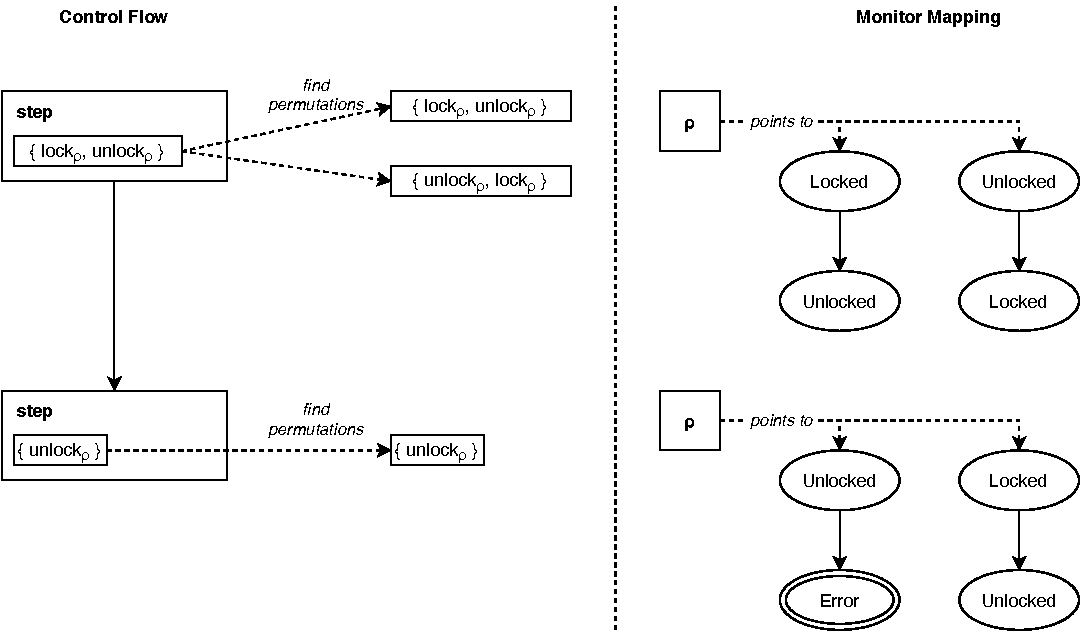
\includegraphics[width=0.85\textwidth]{implementation/figures/permutation-copy}
    \caption{An illustration of the exploration of all effect orderings and how copies of an instantiated double-unlock monitor changes state given these effect orderings, leading to a possible bug being discovered in one effect ordering, but not the other. The control flow graph is shown on the left. On the right I show execution fragments of two double-unlock monitors as defined in \ref{monitor-template-section}.}
    \label{permutation-copy}
\end{figure}

\newpar If the first scenario occurs, a possible bug is definitely present, and exploration can stop. If the second scenario occurs, a possible bug is definitely \underline{not} present, and exploration can continue. If the third scenario occurs, it is unknown whether a possible bug is present, and more information is needed. This extra information is obtained by the inlining the given program point to gain more information regarding the order of effects and applying the effects to the transition function of the monitors once more, making it possible to determine whether a possible bug is present or not. Early use of inlining or inlining of every function leads to the Linux kernel libraries being inlined into the code under analysis, leading to false positives. Inlining is therefore only used when it will benefit the precision of the analysis. 

\newpar The region monitors are instantiated upon and the copies of these monitors are stored in a map from a region to the list of copies. This can be formalized as the function $m: region \rightarrow { [checker\_state] }$ where $ checker\_state $ is the internal state of the monitor automata. Using this map it is possible to apply each permutation of effects and fold this list of effects into a modified map with possibly altered automata states for their corresponding regions. The resulting map can be explored in order to find any accepting states of monitor automata for a given region. 

\newpar Monitors are instantiated whenever a new region is encountered and are then stored in this map. If a given region is already present in the map, then the current state of the monitor(s) monitoring the region are applied on the transition function of the monitor(s). If the region is not already present in the map, a monitor is instantiated for each effect happening in the program point where this region was encountered. Given that the map maps a region to the state of monitor automata, the length of the map will never be larger than the number of regions in the input source file. The size of the set of possible monitor automata states for a given region depends on the effects of a statement operating on a given region, though this can be improved by filtering effects, as we will see shortly. 

\newpar Given a large number of possible effects of a statement the resulting set of permutations of these effects will naturally grow. A set of $N$ effects will result in $N!$ permutations; in other words, the number of monitor states for a given region will therefore in the worst case be $|\mathit{effects}|!$. This $N$ can be reduced by only applying effects to monitors which are of interest, namely effects which are in the alphabet, $\sum$, of the monitor template definition. Effects are only applied to the monitors monitoring a region if the alphabet of the monitor in question accepts this effect, in other words utilizing the product construction inference rules defined in Chapter \ref{control-flow-section}.  Filtering effects caused by a program point to only include elements in $\sum$ greatly reduces the number of monitors states, though this is inherently dependent on the template definition. Definitions with a restricted alphabet will perform better. 

\newpar The full implementation of monitor templates therefore works by:

\begin{itemize}
    \item Taking a source file and a function declaration within that source file, both provided by EBA
    \item Extracting information about the provided function and verifies that the function is non-static
    \item Invoking the CFG-generation of EBA of the provided function
    \item Exploring the effect CFG provided by EBA while invoking the transition function of monitor templates
    \item Filtering the resulting map of monitor states
    \item Pretty-printing the results and returning these to EBA, in turn outputting the results 
\end{itemize}

\newpar The implementation of the exploration of control flow, finding states and adding these states to the map can be seen in Figure \ref{explore_tree-implementation}. This \texttt{explore\_paths} function takes a control flow graph generated by EBA and an initially empty map as input parameters and results in a map of all inferred regions and the resulting monitor states for these regions. This is accomplished by recursively exploring the tree-like control flow graph and depending on the encountered program point, applies the possible effects of the program point on the transition function of the instantiated monitor, \texttt{A}. The resulting state(s) are then added to the map. 

% \begin{figure}[H]
%     \centering
%     \begin{minted}{ocaml}
%     let rec explore_paths path map = 
%         let p = path() in
%         match p with
%         | Seq(step, remaining) -> 
%             let apply_transition effect map = 
%                 let region = get_region effect in 
%                 match region with 
%                 | Some r -> 
%                     let result = Map.find_default [A.initial_state] r map in 
%                     let m = List.fold_left 
%                         (fun acc s -> A.transition s effect step :: acc)
%                         [] result in
%                     Map.add r m map
%                 | None -> map
%             in
%             let input = EffectSet.filter is_in_transition_labels step.effs.may 
%                 |> EffectSet.to_list in
%             if List.is_empty input then explore_paths remaining map 
%             else 
%                 (*  Find all permutations of effects e.g. {{lock, unlock} 
%                     -> {{lock, unlock}, {unlock, lock}} *)
%                 let permutations = permute input in 
%                 let map = List.fold_left (fun map effects ->
%                         (*  For each effect in a permutation, apply the transition, 
%                             and add the result to the map. *)
%                         List.fold_left (fun map effect -> apply_transition effect map) 
%                             map effects
%                     ) map permutations in
%                 explore_paths remaining map
%         | Assume(_, _, remaining) -> 
%             explore_paths remaining map
%         | If(true_path, false_path) -> 
%             let true_branch = explore_paths true_path map in
%             let false_branch = explore_paths false_path map in 
%             Map.merge true_branch false_branch
%         | Nil -> map
%     \end{minted}
%     \caption{The implementation of the EBA control flow while keeping track of states for regions. This function takes a control flow graph generated by EBA and an initially empty map as input parameters and results in a map of all inferred regions and the resulting monitor states for these regions.}
%     \label{explore_tree-implementation}
% \end{figure}

\begin{figure}[H]
    \centering
    \begin{algorithm}[H]
    \begin{algorithmic}
        \Function{explore\_paths} {$tree\_node$, $map$} 
            \If {$tree\_node$ is $\mathit{Nil}$}    
                \State{\Return $map$}
            \ElsIf {$tree\_node$ is $\mathit{If}(t, f)$}
                \State{$true\_branch \gets $ \Call{explore\_paths}{t}}
                \State{$false\_branch \gets $ \Call{explore\_paths}{f}} 
                \State{\Return \Call{merge}{$true\_branch$, $false\_branch$}}
            \ElsIf {$tree\_node$ is $\mathit{Seq}(step, next)$}
                \State{effects $\gets$ step.effects}
                \If{\Call{is\_empty}{effects}}
                    \Return{\Call{explore\_paths}{next, map}}
                \EndIf
                \State{permutations $\gets$ \Call{find\_permutations}{effects}}
                
                \State{\Call{for each effect in each permutation}{\Call{apply\_transition} {effect, map}}}
            \EndIf      
        \EndFunction
        \\
        \Function{apply\_transition} {effect, map}
            \State{region $\gets$ effect.region}
            \State{previous\_states\_for\_region $\gets$ \Call{find\_default}{[initial\_state], region, map}}
            \State states $\gets$ \Call{for each previous state}{\Call{transition} {state, effect}}
            \State{\Return {\Call{add}{map, region, states}}}
        \EndFunction
        \\
        \State{tree $\gets $\Call{generate\_tree} {input\_file}}
        \State{map $\gets $ \Call{explore\_paths}{tree}}
    \end{algorithmic}
    \end{algorithm}
    \caption{Pseudocode illustrating an implementation of the EBA control flow while keeping track of states for regions. This function takes a control flow graph generated by EBA and an initially empty map as input parameters and results in a map of all inferred regions and the resulting monitor states for these regions.}
    \label{explore_tree-implementation}
\end{figure}

\newpar When all paths in the CFG tree structure have been explored, the regions which map to accepting states along with their location and traces are extracted from the mapping and presented to the user as possible bugs.  

\newpar On-the-fly exploration is used since the design of EBA necessitates exploring effects when they are encountered due to performance reasons \cite{Abal2017EffectiveBF}. On-the-fly exploration has been used for ease-of-implementation by following the existing convention of the EBA implementation and for performance reasons. The exploration finds the product construction of the control flow graph and monitor on a step-by-step basis by application of the transition function of a monitor and the information stored in a program point in the control flow graph. The resulting state pair is the product construction of the control flow graph and monitor as decribed in Chapter \ref{monitor-template-section}. 

\newpar The monitor state in the second element of this pair is, as mentioned previously, added to the region and state map in order to track monitor states for regions. The product construction is built step-by-step, but the complete product construction is not saved for later use, as the elements of interest in the resulting pair is the found monitor state. The inference rules defined in Chapter \ref{monitor-template-section} for constructing the product, state that a transition --- the exploration of the program points --- will change the state of the control flow graph, but possibly leave the monitor state in its current state if the effects of a program point are not in the transitions of the monitor. This is reflected in the implementation, where monitors remain in their current state given an input that the monitor does not operate on. Therefore, even though the product construction is not stored or presented explicitly in the implementation, it is still constructed albeit step-by-step and is in a partial state on a given program point.

\newpar Consider the illustration in Chapter \ref{monitor-template-section}, with the relevant part of this illustration shown in Figure \ref{cfg_unlock-product-partial}. When exploring the control flow graph, on encountering the effect \texttt{unlock} and region $\rho$, a monitor is instantiated for $\rho$ in the unlocked state. If a given effect is not in the transitions of the monitor, as seen when encountering the effect \texttt{write}, the exploration continues onto the next program point, implicitly changing the state of the control flow graph by transitioning onto the next node in the graph, while leaving the monitor in its previous state as the inference rules in Chapter \ref{monitor-template-section} state. When encountering an \texttt{unlock} effect, which is in the transitions of the monitor, the monitor will change state to an error state. This corresponds to the defined product construction, though instead of constructing the entire product, this partial product is found on-the-fly. 

\begin{figure}[H]
    \centering
    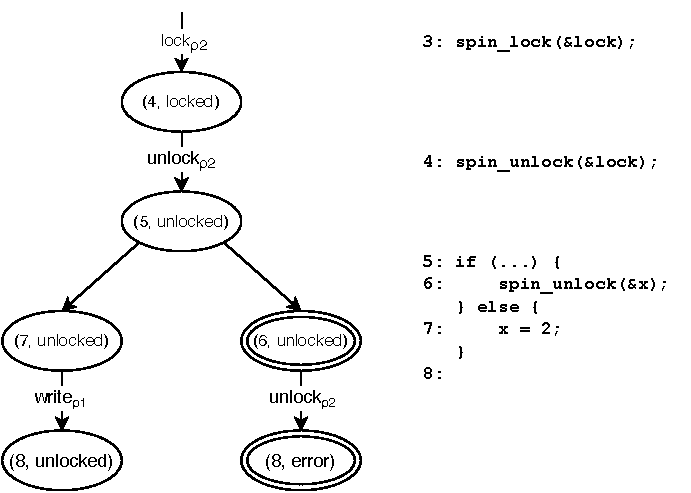
\includegraphics[width=0.5\textwidth]{implementation/figures/cfg_unlock-product-partial}
    \caption{An illustration of the partial product construction of a double-unlock monitor automata and a control flow, based on Figure \ref{cfg_unlock-product}.}
    \label{cfg_unlock-product-partial}
\end{figure}

\subsection{Implementing Monitor Templates as Extensions to EBA}
\label{integration-into-eba}

\noindent In order to implement a new bug checker in EBA, the implementation has to conform to the structure set up by the framework of how these checkers should behave. Furthermore, OCaml signatures must be defined for these checkers in order to allow the framework to instantiate the checkers on the inferred regions of an input program. Specifying a signature which all automata-based checkers must conform to ensures that the automata expose the required state transition functions for them to run. This section will describe how this has been accomplished.  

\newpar Monitor automata are used to detect bugs over control flow graphs. The control flow graph is provided by the EBA framework, while the monitor automata have been defined and implemented as part of this thesis. These bug checkers must conform to the existing signatures of EBA in order to allow the framework to instantiate a given bug checker after which an abstract representation of the input source file is passed to the instantiated checker. 

\newpar A signature which allows instantiation of monitor automata bug checkers has been defined as part of this thesis. This signature is then implemented in order to let EBA instantiate the implemented checker. A function, \texttt{check}, is the only requirement for implementing this signature and takes two parameters after which it returns a list of strings for each detected possible bug in the input source file as expected by the EBA framework. These parameters are the abstractions of the input file and each global function defined in this file, both of which are passed to the function by the framework. This mimics the implementation of the existing CTL checkers in EBA and allows for easy integration into the framework. A snippet of the \texttt{Make} signature can is shown in Figure \ref{make-signature}.

\begin{figure}[H]
    \centering
    \begin{minted}{ocaml}
    module type S = sig
        type result
        val check : AFile.t -> Cil.fundec -> result list
        val filter_results : result list -> result list
        val stringify_results : result list -> string list
    end

    module Make (A : AutomataSpec) : S = struct
        type result = A.checker_state
        let check file declaration = ...
        let filter_results matches = A.filter_results matches
        let stringify_results matches = ...
    end
    \end{minted}
    \caption{A snippet of the \texttt{Make} module and its use of dependency injection for the instantiation of a checker conforming to the \texttt{AutomataSpec} signature.}
    \label{make-signature}
\end{figure}

\newpar The aforementioned signature is implemented as a module, \texttt{Make}, which is used by EBA in order to run automata bug checkers conforming to an automata signature. The \texttt{Make} module expects an implementation of this \texttt{AutomataSpec} signature. 

\noindent The implementation of \texttt{check} initiating the generation of the control flow abstraction using EBA can be seen in Figure \ref{check-implementation}. This function can be summarized as:

\begin{itemize}
    \item Taking a source file, \texttt{file} and a function declaration, \texttt{declaration} within that source file provided by EBA
    \item Extracting information, \texttt{variable\_info}, about the provided function and verifies that the function is non-static
    \item Invoking the \texttt{paths\_of} CFG-generation of EBA of the function
    \item Exploring the effect CFG provided by EBA, \texttt{explore\_paths}, while invoking the transition function of a monitor template
    \item Filtering the resulting map of regions and monitor states
    \item Pretty-printing the results and returns these to EBA which in turn shows the results 
\end{itemize}

\begin{figure}[H]
    \centering
    \begin{minted}{ocaml}
    let check file declaration =
        let variable_info = Cil.(declaration.svar) in
        match variable_info.vstorage with 
        | Static -> L.of_list []
        | _ ->
            let _, global_function = Option.get(AFile.find_fun 
                file variable_info) in
            let path_tree = paths_of global_function in
            let results = explore_paths global_function path_tree 
                Map.empty true in 
            let states = Map.values results in
            let matches = Enum.fold (fun acc m -> 
                (List.filter A.is_accepting m) @ acc) [] states in
            let matches_reversed = List.rev matches in 
            let function_name = Cil.(variable_info.vname) in 
            let pp = List.map (fun m -> A.pp_checker_state m function_name) 
                matches_reversed in
            let pp_list = List.map (fun m -> PP.to_string m) pp in
            L.of_list pp_list
    \end{minted}
    \caption{The implementation of \texttt{check} initializing the control flow generation using EBA.}
    \label{check-implementation}
\end{figure}

\newpar Nodes in the CFG structure provided by EBA can be of one of four different types, each representing the input statement. Nodes representing if-statements in the source input result are \textit{If}-nodes in the tree, containing two branches. If an If-node is discovered, the two branches from that node are explored and the union of the resulting states is found. Nodes representing the end of a branch are \textit{Nil}-nodes in the tree. Nodes representing assumptions made after if-statements are either true or false are \textit{Assume}-nodes, but are not used in this work since all branches are explored. Finally all other statements are represented as \textit{Seq}-nodes, which contain information about the shapes and effects of statements. These \textit{Seq}-nodes are of interest, since they allow analysis on effects. Seq-nodes contain a \textit{step} which models a statement in the input source code. When a \textit{Seq}-node is discovered in the tree, the --- possibly multiple --- effects of its containing step are explored. 

% \begin{figure}[H]
%     \centering
%     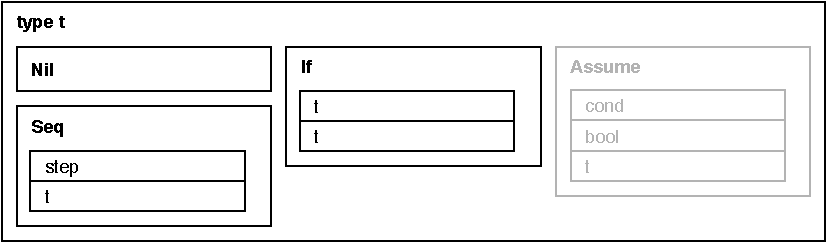
\includegraphics[width=0.9\textwidth]{implementation/figures/node}
%     \caption{An illustration of the CFG node types found in EBA.}
%     \label{cfg-nodes}
% \end{figure}

% \begin{figure}[H]
%     \centering
%     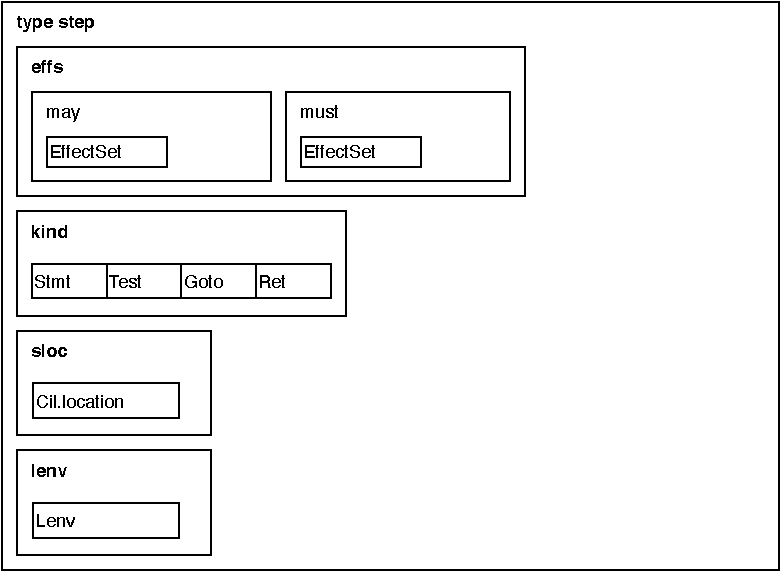
\includegraphics[width=0.8\textwidth]{implementation/figures/step}
%     \caption{An illustration of the step type and its containing structures found in EBA.}
%     \label{cfg-step}
% \end{figure}

\newpar The implementation of a given monitor automata is passed to the aforementioned \texttt{Make} module and is then used to evaluate states based on the effects of regions. The signature of the monitor automata specifies a \texttt{state} as a discriminated union type, describing the possible states of the automata as well as a transition function, \texttt{transition}, which takes a previous state of the monitor along with an input effect. 

\newpar In order to provide the user with detailed error reports this state is encapsulated in a \texttt{checker\_state} structure which keeps track of the current trace through the CFG along with granular location details for discovered possible bugs. Providing this information requires that the current CFG node must also be passed to the automata, due to the architecture of the EBA framework. The full signature for the transition function is therefore $transition: \mathit{checker\_state} \rightarrow \mathit{effect} \rightarrow \mathit{step} \rightarrow \mathit{checker\_state}$. No references to instantiated monitor moudules are stored in the map, merely the current states of monitors. 

\begin{figure}[H]
    \centering
    \begin{minipage}[t]{0.45\textwidth}
    \begin{minted}[breaklines]{ocaml}
    type state = 
        | Locked
        | Unlocked
        | Error of Effects.e
    \end{minted}
    \end{minipage}
    \hspace*{0.05\textwidth}
    \begin{minipage}[t]{0.45\textwidth}
    \begin{minted}[breaklines]{ocaml}
    type checker_state = {
        current_state: state;
        trace: step list;
        matches: step list;
    }
    \end{minted}
    \end{minipage}
    \caption{An illustration of the \textit{state} and \textit{checker\_state} structures for a double-unlock monitor.}
    \label{checker-state}
    \end{figure}

\newpar A concrete example of a $checker\_state$ structure can be seen in Figure \ref{checker-state}. This transition function in other words operates on an effect which is part of the set of effect types and results in a new monitor state which is part of the set of possible states defined within the monitor, reflecting the definition of a monitor template seen in Section \ref{monitor-template-section}. A concrete example of an implementation of the transition function can be seen in Figure \ref{transition-implementation}. 

\begin{figure}[H]
    \centering
    \begin{minted}{ocaml}
        let transition previous input step = 
            let next new_state = with_previous previous new_state step in
            let previous_state = previous.current_state in 
            match previous_state with 
            | Unlocked ->
                (match input with 
                | Mem(Lock, _)      -> next Locked
                | Mem(Unlock, _)    -> next (Error input)
                | _                 -> next previous_state
                )
            | Locked ->
                (match input with 
                | Mem(Unlock, _)    -> next Unlocked
                | _                 -> next previous_state
                )
            | Error _               -> next previous_state
    \end{minted}
    \caption{The implementation of the transition function of the double-unlock monitor template definition.}
    \label{transition-implementation}
\end{figure}

\newpar This implementation has been chosen for performance reasons and simplicity, since the transition function of a monitor does not change after it has been defined and can therefore be implemented as a performant static function. Storing only previous states and taking this previous state into consideration in the implementation of transition functions results in a lower memory footprint and possibly higher readability of the implementation since an alternative implementation, e.g. based on dynamically assigning transitions to an internal map within the monitor, would increase the memory footprint and possible make it hard to track what the possible states for a given monitor are for the reader.

\newpar It became apparent during testing of the implementation that the loop unrolling by EBA resulted in false positives being detected. The unrolling of loops in EBA causes false positives since monitor templates register loops as multiple repetitions of the same effect in a path due to the way unrolled loops are represented. An effect $e$ of a program point in a loop will be unrolled to a path of $N$ length with each program point in that path having the effect $e$. Figure \ref{unrolling-false-positive} shows an illustration of this problem. In the case of unlocks, any unlock happening within a loop is therefore reported as a double unlock, since the path under examination will have $N$ unlocks in sequence, due to the structure of the effect-CFG. This $N$ is configurable in EBA, though only with an $N > 1$. Filtering has been implemented so such paths are detected and filtered, improving the quality of the output, in turn making the implementation more desirable to use \cite{false-positives}. This filtering examines the trace of all positives resulting of checking a file, and will remove any positive which has a trace consisting of the same program point, in effect detecting the original unrolled loop path. Furthermore, kill-region detection has also been implemented in line with the kill-region detection implementation found in the existing CTL checkers of EBA \cite{Abal2017EffectiveBF}. Kill-region detection as well as detection and filtering of undesirable effects of the loop unrolling found in EBA has reduced the amount of false positives significantly, in turn improving the output of bug checkers significantly. 

\begin{figure}[H]
    \centering
    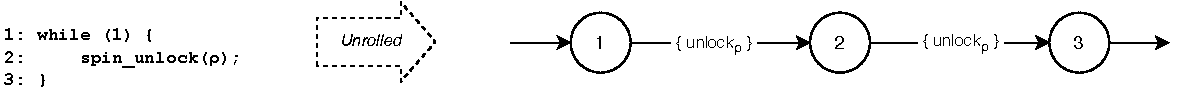
\includegraphics[width=0.95\textwidth]{implementation/figures/unrolling-false-positive}
    \caption{An illustration of the unrolling of loops found in EBA, resulting in a path containing the same effect of a program point in a loop repeated in sequence. An unlock effect of a program point in a loop will be unrolled to a path of length $N = 2$ with each program point in that path having the same effect.}
    \label{unrolling-false-positive}
\end{figure}